\documentclass{report}
\usepackage[spanish]{babel}
\usepackage{natbib}
\usepackage{url}
\usepackage[utf8]{inputenc}
\usepackage{amsmath}
\usepackage{graphicx}
\graphicspath{{images/}}
\usepackage{parskip}
\usepackage{fancyhdr}
\usepackage{vmargin}
\usepackage{subfig}
\usepackage[hidelinks]{hyperref}
\usepackage{enumerate}
\usepackage[usenames]{color}
\usepackage{soul}
\usepackage{float}
\usepackage[T1]{fontenc}
\usepackage{verbatim}
\usepackage{multicol}
\usepackage{listings}
\usepackage{multirow}
\usepackage{booktabs}

\setmarginsrb{3 cm}{2.5 cm}{3 cm}{2.5 cm}{1 cm}{1.5 cm}{1 cm}{1.5 cm}

\title{\textsc{Reporte Revisión Sistemática\\Gamificación en la E-Learning}}
\author{Luis Angel Hernández Lázaro}
\date{\today}

\makeatletter
\let\thetitle\@title
\let\theauthor\@author
\let\thedate\@date
\makeatother

\pagestyle{fancy}
\fancyhf{}
\rhead{\theauthor}
\lhead{\thetitle}
\cfoot{\thepage}
\setcounter{secnumdepth}{5}

\begin{document}

%%%%%%%%%%%%%%%%%%%%%%%%%%%%%%%%%%%%%%%%%%%%%%%%%%%%%%%%%%%%%%%%%%%%%%%%%%%%%%%%%%%%%%%%%

\begin{titlepage}
	\centering
    \vspace*{0.5 cm}
    
    \begin{figure}
		\centering
		\subfloat{
			\label{logoCimat}
		    
\includegraphics[scale = 0.15]{images/0cover/logoCimat.png}
		}
	\end{figure}
    \textsc{\LARGE Centro de Investigación en Matemáticas A.C.}\\[1.0 cm]
	\textsc{\Large Maestría en Ingeniería de Software}\\[0.5 cm]
	\textsc{\large Métodos y Técnicas de Investigación \\ Orientadas a la Ingeniería de Software\\{-}\\Estudio Guiado I\\Dra. Mirna Ariadna Muñoz Mata}\\[0.5 cm]
	\rule{\linewidth}{0.2 mm} \\[0.4 cm]
	{ \huge \bfseries \thetitle}\\ \textsc{\large Luis Angel Hernández Lázaro}
	\rule{\linewidth}{0.2 mm} \\[1.5 cm]
	
	\begin{minipage}{0.5\textwidth}
		\begin{flushleft} \large
			\emph{Correo:}\\
			luis.hernandez@cimat.mx
		\end{flushleft}
	\end{minipage}~
	\begin{minipage}{0.4\textwidth}
		\begin{flushright} \large
		\end{flushright}
	\end{minipage}\\[2 cm]
		
	{\large \thedate}\\[2 cm]
 
	\vfill
	
\end{titlepage}

%%%%%%%%%%%%%%%%%%%%%%%%%%%%%%%%%%%%%%%%%%%%%%%%%%%%%%%%%%%%%%%%%%%%%%%%%%%%%%%%%%%%%%%%%

\tableofcontents
\pagebreak

%%%%%%%%%%%%%%%%%%%%%%%%%%%%%%%%%%%%%%%%%%%%%%%%%%%%%%%%%%%%%%%%%%%%%%%%%%%%%%%%%%%%%%%%%
\chapter{Inicio}
    
    \section{Introducción}
    El presente reporte está creado con la finalidad de mostrar los resultados de la revisión sistemática desarrollada durante la materia de Métodos y Técnicas de Investigación Orientadas a la Ingeniería de Software impartida por la Dra. Mirna Ariadna Muñoz Mata. La revisión sistemática se ha centrado en el tema de Gamificación, principalmente en las técnicas o métodos aplicadas en el área de la educación.\\
    
\chapter{Revisión Sistemática}

    \section{Introducción}
    Se ha elegido este tema debido al interés en el área para aplicar técnicas o métodos de gamificación en la educación, para motivar el aprendizaje de los estudiantes y mejorar su desempeño académico.\\

    AGREGAR PEQUEÑAS RESEÑAS DE LA GAMIFICACIÓN EN LA EDUCACIÓN A PARTIR DE LOS ESTUDIOS PRIMARIOS 
    Y DESCRIBIR QUE ABORDA LA REVISIÓN SISTEMÁTICA    
    
    ...Explicar brevemente cada punto...
    
    El documento de la revisión sistemática se encuentra estructurado de la siguiente manera:
    \begin{description}
        \item[Background] Términos y conceptos acerca de gamificación y educación, algo más de teoría.
        \item[El proceso de la Revisión Sistemática] Descripción de las etapas para el desarrollo de la revisión sistemática.
        \begin{description}
            \item[Planeación] Necesidad, preguntas, protocolo
            \item[Ejecución] Búsqueda, estudios primarios.
            \item[Reporte] Análisis de la información.
        \end{description}
        \item[Conclusión] Conclusión de la revisión sistemática.
    \end{description}    
    
    \section{Background}\label{back}
        ...EN PROCESO AL TERMINAR LA LECTURA DE POR LO MENOS 5 ESTUDIOS PRIMARIOS
    
    \section{El Proceso de la Revisión Sistemática}
    
    Una revisión sistemática se basa en el objetivo para recolectar estudios de un tema en especial a investigar, originando la búsqueda de nuevos conocimientos para nuestra formación académica. ``Una Revisión sistemática de la literatura permite identificar, evaluar, interpretar y sintetizar todas las investigaciones existentes y relevantes en un tema de interés en particular'' \textbf{PONER CITA DEL ARTICULO}.\\
        En la tabla \ref{table:stepsSystematicReview} se muestran las etapas principales con sus respectivos pasos, que conforman una revisión sistemática. Para estimular la creación de esta revisión sistemática, se va a investigar cuales son los resultados de las técnicas de gamificación aplicadas en la educación.\\
Algunas de las características que diferencian una revisión sistemática de una revisión de la literatura convencional son\textbf{PONER CITA DEL ARTÍCULO}:
    \begin{enumerate}    
    	\item La revisión sistemática comienza por definir un protocolo de revisión que especifica la(s) pregunta(s) de investigación abordados y los métodos que serán usados para realizar la revisión.
    	\item Las revisiones sistemáticas son basadas definiendo una estrategia de búsqueda que tiene como objetivo detectar la mayor cantidad de literatura relevante posible.
	    \item Las revisiones sistemáticas documentan sus estrategias de búsqueda para que los lectores puedan evaluar su rigor y exahustividad y la repetitividad del proceso.
    	\item Las revisiones sistemáticas requieren criterios de inclusión y criterios de exclusión explícitos para evaluar cada estudio primario potencial.
	    \item Las revisiones sistemáticas especifican la información para obtener cada uno de los estudios primarios incluyendo los criterios de calidad para evaluar cada estudio primario.
    \end{enumerate}
    \begin{table}
        \begin{center}
            \caption{Pasos de la Revisión Sistemática}
            \label{table:stepsSystematicReview}
            \begin{tabular}{| p{5cm} | l |}
                \toprule
                \hline 
                \multicolumn{1}{|c|}{\textbf{Etapa}} & \multicolumn{1}{|c|}{\textbf{Paso}}\\
                \hline
                \multicolumn{1}{|c|}
                    {\multirow{4}{*}
                        {\begin{tabular}[c]{@{}c@{}}
                            Planificación de\\ la Revisión
                        \end{tabular}}
                    } & Identificación de la necesidad para realizar la revisión.\\ \cline{2-2} 
                    \multicolumn{1}{|c|}{} & Especificación de la(s) pregunta(s) de investigación.\\ \cline{2-2} 
                    \multicolumn{1}{|c|}{} & Desarrollo del protocolo de revisión.\\ \cline{2-2} 
                    \multicolumn{1}{|c|}{} & Evaluación del protocolo de revisión.\\ 
                \hline
                \multicolumn{1}{|c|}
                    {\multirow{5}{*}
                        {\begin{tabular}[c]{@{}c@{}}
                            Ejecución de\\ la Revisión
                        \end{tabular}}
                    } & Identificación de la investigación.\\ \cline{2-2} 
                    \multicolumn{1}{|c|}{} & Selección de estudios primarios.\\ \cline{2-2} 
                    \multicolumn{1}{|c|}{} & Evaluación de la calidad de los estudios.\\ \cline{2-2} 
                    \multicolumn{1}{|c|}{} & Extracción y monitoreo de datos.\\ \cline{2-2} 
                    \multicolumn{1}{|c|}{} & Sintetizar los datos.\\ 
                \hline
                \multicolumn{1}{|c|}
                    {\multirow{3}{*}
                        {\begin{tabular}[c]{@{}c@{}}
                            Ejecución de\\ la Revisión
                        \end{tabular}}
                    } & Especificación de los mecanismos de difusión.\\ \cline{2-2} 
                    \multicolumn{1}{|c|}{} & Formateo del informe principal.\\ \cline{2-2} 
                    \multicolumn{1}{|c|}{} & Evaluación del reporte.\\ 
                \hline
            \end{tabular}
        \end{center}
    \end{table}
    
    \subsection{Planeación de la Revisión Sistemática}
     Al realizar nuestra revisión sistemática es importante la etapa de la planeación, para establecer las actividades a ejecutar, de esta forma definimos nuestro marco de trabajo durante la ejecución de la revisión sistemática, es importante realizar la planeación de forma correcta, así como la identificación de la necesidad de la revisión para evitar caer en problemas durante su ejecución.\\
    	En esta primera etapa, la actividad más importante a tener en cuenta es la definición de la(s) pregunta(s) de investigación, puesto que son el punto clave para el desarrollo de nuestra investigación.\\
    	Como parte de la definición de nuestro Objetivo General del estudio tenemos:
        \begin{enumerate}
        	\item Definir el estado del actual del uso de técnicas de Gamificación en la educación tradicional (aula - alumno - profesor), para descubrir las diferentes técnicas de Gamificación para implementarlas en la educación.
        \end{enumerate}
Los objetivos Específicos del estudio son:
        \begin{enumerate}
        	\item Definir el estado del arte de la Gamificación en E-Learning.
        	\item Revisar las estrategias o técnicas de Gamificación implementadas en el área de la educación.
        	\item Comparar la aplicación técnicas de gamificación implementadas en educación.
        \end{enumerate}

    	    \subsubsection{Identificación de la Necesidad de la Revisión Sistemática} \label{needs}
    	    
            Hoy en día la Gamificación es un tema que esta siendo aplicado más allá de los juegos que tradicionalmente conocemos, la aplicación de técnicas para gamificación pueden ser variadas dependiendo del área donde se trabaje. Entonces, es importante conocer si las técnicas y métodos de Gamificación desarrollados para la educación pueden ser aplicados en entornos de la educación en línea (E-Learning). \\
           OBTENER LAS REFERENCIAS DE ESTUDIOS PRIMARIOS ...EN PROCESO DE LECTURA
            
    	    \subsubsection{Especificación de las Preguntas de Investigación}
            La revisión sistemática es desarrollada para identificar y conocer el estado del arte referente a la Gamificación en el área de la educación. Sin embargo también se desea conocer como ha sido aplicada la Gamificación en diferentes áreas para promover el aprendizaje, con el objetivo de identificar cuál ha sido su efectividad en la implementación de técnicas de Gamificación. En la Tabla \ref{table:researchQuestions} se muestran las preguntas de investigación formuladas para esta investigación, las cuales serán contestadas al realizar esta revisión sistemática.\\
            Para la formulación de las preguntas se apoyó en el método PICOC (Población, Intervención, Comparación, Salidas y Contexto), la estructura PICOC permitió identificar y aclarar nuestras preguntas de investigación para crear un ambiente de trabajo más detallado de nuestra área de investigación. A continuación se detalla cuales son nuestros elementos contemplados en la estructura PICOC:\\
            \begin{description}
                \item[Población]: Técnicas o Métodos de Gamificación en el área de la Educación
                \item[Intervención]: Técnicas o Métodos de Gamificación en Educación Tradicional.
                \item[Comparación]: Técnicas o Métodos de Gamificación en E-Learning.
                \item[Salidas]: Comparación acerca de las técnicas de gamificación implementadas.
                \item[Contexto]: Académico
            \end{description}
            \begin{table}
                \begin{center}
                    \caption{Preguntas de Investigación}
                    \label{table:researchQuestions}
                    \begin{tabular}{| l | p{6cm} | p{6cm} |}
                        \toprule
                        \hline
                        \multicolumn{1}{|c|}{\textbf{RQ\#}} & \multicolumn{1}{|c|}{\textbf{Pregunta}}  & \multicolumn{1}{|c|}{\textbf{Objetivo}} \\
                        \hline
                        RQ1 & ¿Qué elementos de gamificación son usados en la educación? & Identificar los elementos de Gamificación existentes, en particular en la educación. \\
                        \hline
                        RQ2 & ¿Qué tipo de estudios de investigación aplican gamificación en la educación? & Descubrir los trabajos que han sido desarrollados para aplicar la gamificación en la educación. \\
                        \hline
                        RQ3 & ¿Qué técnicas de gamificación han sido más efectivas? & De las técnicas existentes cuales han tenido resultados positivos en la educación y porque. \\
                        \hline
                        RQ4 & ¿La gamificación en e-learning promueve el aprendizaje? & De de las técnicas de gamificación cuales se han aplicado para el área de la educación.\\
                        \hline
                        RQ5 & ¿En qué contextos ha sido investigada la gamificación? & Que experiencias se han tenido en el uso de gamificación.\\
                        \hline
                    \end{tabular}
                \end{center}
            \end{table}
            
            \subsubsection{Evaluación del Protocolo de Revisión}

            Como parte de la evaluación del protocolo se realizaron revisiones con el Dr. José Arturo Mora Soto asesor para realizar esta investigación. Una de las observaciones para mejorar la calidad de los estudios primarios fue la actualización de la palabra clave (keyword) <<Serious Game>> por <<Serious Games>>, palabra clave que permitió la creación de una cadena de búsqueda aplicada a en las bibliotecas digitales. \\

        \subsection{Ejecución de la Revisión}
    
        Ahora que hemos establecido cuales son nuestras preguntas de investigación y el protocolo de investigación, comenzamos la etapa de ejecución. Durante la ejecución de la revisión sistemática debemos respetar el procedimiento establecido en el protocolo.
    
            \subsubsection{Selección de las Fuentes de  Investigación}
    
            La búsqueda para encontrar los estudios más relevantes se realizó en bibliotecas digitales haciendo uso de las cadenas de búsqueda con las siguientes palabras clave:
            \begin{enumerate}
                \item Gamification
                \item Gamify
                \item Serious Games
                \item Education
                \item E-Learning
            \end{enumerate}       
            En la Tabla \ref{table:SearchString} se muestran las cadenas de búsqueda aplicadas a las bibliotecas digitales, como se puede notar las cadenas de búsqueda están formadas por las palabras claves de nuestra investigaciones y se combinaron mediante el uso de los conectores lógicos ``OR''{ }y ``AND''.    
            \begin{table}
                \begin{center}
                    \caption{Cadenas de Búsqueda}
                    \label{table:SearchString}
                    \begin{tabular}{| p{1.5cm} | p{12.5cm} |}
                        \toprule
                        \hline
                        \multicolumn{1}{|c|}{\textbf{Núm}} & \multicolumn{1}{|c|}{\textbf{Cadena de Búsqueda}} \\
                        \hline
                        SS1 & ( ``Gamification''{ }AND (``Education''{ }OR ``E-Learning''{ }) )\\
                        \hline
                        SS2 & ( ``Serious Games''{ }AND ``Gamification''{ }AND (``Education''{ }OR ``E-Learning''{ }) )\\
                        \hline            
                        SS3 & ( ``Gamify''{ }AND (``Education''{ }OR ``E-Learning''{ }) )\\
                        \hline
                    \end{tabular}
                \end{center}
            \end{table}
            
            Inicialmente durante nuestra investigación se tenían contempladas 8 Bibliotecas Digitales para la aplicación de las cadenas de búsqueda, sin embargo durante la evaluación de los bibliotecas digitales 2 fueron excluidas de la selección: JSTOR debido al poco contenido ofrecido en temas de gamificación y e-learning y Google Scholar debido a la excesiva cantidad de resultados obtenidos para nuestras cadenas de búsqueda; ambas fueron excluidas para la recolección de estudios relevantes con el propósito de recolectar estudios relevantes sin mucha perdida de tiempo durante su búsqueda. De igual manera se encontraron casos donde un estudio relevante estaba presente en otra de las fuentes seleccionadas.\\ En la tabla \ref{table:libraries} se muestra la lista de bibliotecas digitales inicialmente contempladas y las bibliotecas digitales donde se llevo a cabo la aplicación de nuestras cadenas de búsqueda.
            \begin{table}
                \begin{center}
                    \caption{Fuentes de Búsqueda}
                    \label{table:libraries}
                    \begin{tabular}{| p{7cm} | p{7cm} |}
                        \toprule
                        \hline
                        \textbf {Fuentes Contempladas en un Inicio} &  \textbf{Fuentes Donde se Realizó la Búsqueda}\\
                        \hline
                        IEEE Xplore Digital Library & IEEE Xplore Digital Library\\
                        \hline
                        ACM Digital Library & ACM Digital Library\\
                        \hline
                        Web of Science & Web of Science\\
                        \hline
                        JSTOR & x\\
                        \hline
                        Scopus & Scopus\\
                        \hline
                        Springer Link & Springer Link\\
                        \hline
                        Elsevier Science Direct & Elsevier Science Direct\\
                        \hline
                        Google Scholar & x\\
                        \hline
                    \end{tabular}
                \end{center}
            \end{table}
    
            \subsubsection{Procedimiento de Selección de los Estudios Relevantes}
    
	        En esta actividad, se describe la manera en la que fueron seleccionados los estudios, después de realizar la búsqueda con nuestras cadenas de búsqueda definidas en la tabla \ref{table:SearchString} aplicadas en las bibliotecas digitales tabla \ref{table:libraries}. Al ejecutar la búsqueda en cada una de las bibliotecas seleccionadas, debemos aplicar nuestros criterios de inclusión y exclusión para destacar los estudios candidatos a convertirse a estudios primarios.\\
    	    Los criterios de inclusión y exclusión permiten acortar el número de resultados y enfocarnos en estudios de nuestro interés, relevantes para nuestra investigación y con un alto impacto de conocimiento. En esta investigación los criterios de inclusión y exclusión se muestran en la tabla \ref{table:criterios}. Cabe mencionar que la búsqueda de estudios se realizo durante el periodo del: 26 al 30 de noviembre del año 2015.\\
        	\begin{table}
                \begin{center}
                    \caption{Criterios de inclusión y exclusión}
                    \label{table:criterios}
                    \begin{tabular}{| p{7cm} | p{7cm} |}
                        \toprule
                        \hline
                        \multicolumn{1}{|c|}{\textbf{Criterios de Inclusión}} & \multicolumn{1}{|c|}{\textbf{Criterios de Exclusión}} \\
                        \hline
                        Incluir artículos donde el título contengan dos términos de nuestras cadenas de búsqueda principalmente ``Gamification''{ }& Excluir todos los artículos que correspondan con los criterios de inclusión definidos.\\
                        \hline
                        Incluir artículos que contengan dentro de sus palabras clave por lo menos dos términos de nuestras cadenas de búsqueda. & Excluir todos los artículos duplicados para eliminar la redundancia de información.\\
                        \hline
                        Incluir artículos donde el resumen presente una relación con la aplicación de técnicas de gamificación. & Excluir artículos que se encuentren en idiomas diferentes al español o ingles.\\
                        \hline
                        . & Excluir artículos que contengan más de 10 páginas, debido a la limitación de tiempo para realizar la RS, con excepción de los artículos que sean de suma importancia para la investigación.\\
                        \hline
                    \end{tabular}
                \end{center}
            \end{table}
            Durante la ejecución de las cadenas de búsqueda, si el artículo encontrado en los resultados solo contenía un término de búsqueda, se procedió a revisar el título para conocer si existía una relación con el tema de nuestra investigación, si el título no proporcionaba un panorama especifico del estudio, se prosiguió a la lectura del abstract (resumen) para determinar si el artículo calificaba como estudio relevante.\\
            A partir de los resultados de nuestras cadenas de búsqueda se muestra la distribución de estudios relevantes en la tabla \ref{table:ResultsSearchString}. La aplicación de las cadenas de búsqueda se realizó de la siguiente manera: se aplicó la cadena SS1, posteriormente la cadena SS2 y por último la cadena SS3 (ver la Tabla de Cadenas de Búsqueda \ref{table:SearchString}); la búsqueda se realizó a las bibliotecas en el orden descrito a continuación:
            \begin{enumerate}\label{jerarquiaBD}
                \item IEEE Xplore Digital Library.
                \item ACM Digital Library.
                \item Web of Science.
                \item Scopus.
                \item Springer Link.
                \item Elsevier Science Direct.
            \end{enumerate}
            \begin{table}
                \begin{center}
                    \caption{Resultados de Cadenas de Búsqueda}
                    \label{table:ResultsSearchString}
                    \begin{tabular}{| p{6cm} | p{1cm} | p{1cm} | p{1cm} | p{4cm} |}
                        \toprule
                        \hline
                        \textbf{Fuente /Cadena} & \textbf{ss1} & \textbf{ss2} & \textbf{ss3} & \textbf{Total por Biblioteca Digital}\\ \hline
                        ACM Digital Library & 123 & 93 & 45 & 261\\ \hline
                        Elsevier Science Direct & 301 & 93 & 27 & 421\\ \hline
                        IEEE Xplore Digital Library & 102 & 4 & 77151\textsuperscript{*} & 106\\ \hline
                        Scopus & 359 & 49 & 11 & 419\\ \hline
                        Springer Link & 736 & 284 & 64 &  1084\\ \hline
                        Web of Science & 139 & 18 & 0 & 157\\ \hline
                        \textbf{Total por Cadena de Búsqueda} & \textbf{1760} & \textbf{541} & \textbf{147} & \textbf{2448}\\ \hline
                    \end{tabular}
                \end{center}
            \end{table}
            Para cada una de las bibliotecas digitales se analizaron los resultados con base en los criterios de inclusión (tabla \ref{table:criterios}) para obtener los estudios relevantes del tema, con la finalidad de pulir la búsqueda previa a la selección de estudios primarios. Los resultados de las cadenas de búsqueda aplicando nuestros criterios de inclusión y exclusión se pueden observar en la tabla \ref{table:ResultsSearchStringOutStandingStudies}.
            \begin{table}
                \begin{center}
                \caption{Resultados de Cadenas de Búsqueda, Estudios Relevantes}
                \label{table:ResultsSearchStringOutStandingStudies}
                    \begin{tabular}{| p{6cm} | p{1cm} | p{1cm} | p{1cm} | p{4cm} |}
                        \toprule
                        \hline
                        \textbf{Fuente /Cadena} & \textbf{ss1} & \textbf{ss2} & \textbf{ss3} & \textbf{Total por Biblioteca Digital}\\ \hline
                        ACM Digital Library & 13 & 4 & 3 & 20 \\ \hline
                        Elsevier Science Direct & 7 & 1 & 0 & 8\\ \hline
                        IEEE Xplore Digital Library & 17 & 1 & 0 & 18\\ \hline
                        Scopus & 0 & 0 & 2 & 2\\ \hline
                        Springer Link & 17 & 2 & 1 &  20\\ \hline
                        Web of Science & 9 & 0 & 0 & 9 \\ \hline
                        \textbf{Total por Cadena de Búsqueda} & \textbf{63} & \textbf{8} & \textbf{6} & \textbf{77}\\ \hline
                    \end{tabular}
                \end{center}
            \end{table}
            Durante la selección de estudios relevantes, existió la repetición de artículos en diferentes bibliotecas digitales, por lo tanto sólo se contemplo un ejemplar de estudio seleccionado por medio de la jerarquía de búsqueda descrita en la sección \ref{jerarquiaBD}. Como resultado de la búsqueda aplicando nuestros criterios de inclusión y exclusión a los estudios, se obtuvo una selección de estudias con probabilidades muy altas de ser un estudio primario. Se puede observar el detalle de la identificación de estudios primarios en la figura \ref{seleccionParte1}.\\            
            \begin{figure}
                \centering
	    	    \subfloat{
    	    	    \label{seleccionParte1}
    	    	    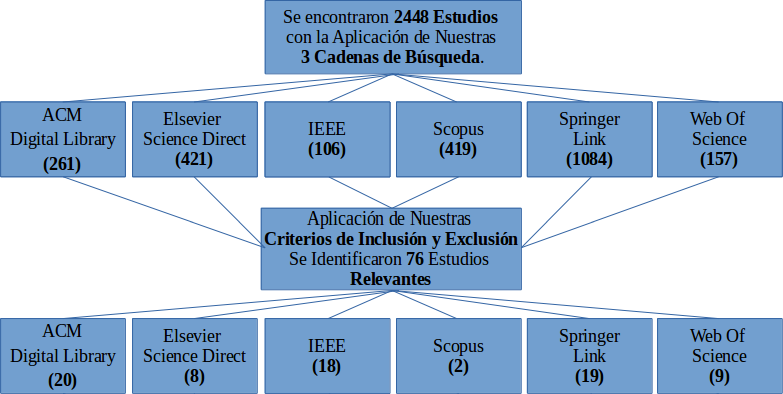
\includegraphics[scale = 0.53]{images/1document/seleccionParte1.png}
        		}
        		\caption{Procedimiento de Selección de Estudios Primarios}
         	\end{figure}
            
            \subsubsection{Evaluación de la Calidad de los Estudios}
            Durante este paso, se aplicaron criterios de selección de inclusión y exclusión para determinar si el estudio encontrado cumple los requisitos para ser tomado en cuenta como estudio primario. A continuación en la Tabla \ref{table:CriteriosInclusionExclusionCalidad}, se muestran los criterios de calidad para seleccionar los estudios primarios.
            
            \begin{table}[H]
                \begin{center}
                    \caption{Criterios de inclusión y exclusión aplicados para la extracción de la Información}
                    \label{table:CriteriosInclusionExclusionCalidad}
                    \begin{tabular}{| p{7cm} | p{7cm} |}
                        \toprule
                        \hline
                        \multicolumn{1}{|c|}{\textbf{Criterios de Inclusión}} & \multicolumn{1}{|c|}{\textbf{Criterios de Exclusión}} \\
                        \hline
                        Incluir información sobre métodos de implementación para establecer estrategias de aprendizaje por medio de ``Gamification''.{ }& Excluir toda la información que no este relacionada con los criterios de inclusión definidos.\\
                        \hline
                        Incluir información que contenga experiencias en la mejora del aprendizaje con ``Gamification''. &{ } \\
                        \hline
                        Incluir información donde se muestren estudios mejoras para el aprendizaje por medio de técnicas de e-learning.\\ \hline
                    \end{tabular}
                \end{center}
            \end{table}
            
            En la figura \ref{seleccionParte2}  se observa el resumen del procedimiento para la selección de estudios primarios, describe la ejecución inicial de las cadenas de búsquedas con un resultado total de 2448 estudios encontrados, al aplicar los criterios de inclusión y exclusión se redujo a 77 estudios relevantes y posteriormente se llevo a la selección de 55 estudios primarios. Para ver la lista completa de estudios primarios puede consultar la Sección de Anexos.
            
            \begin{figure}
                \centering
	    	    \subfloat{
    	    	    \label{seleccionParte2}
    	    	    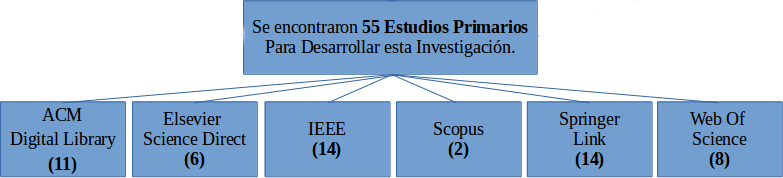
\includegraphics[scale = 0.53]{images/1document/seleccionParte2.png}
        		}
        		\caption{Procedimiento de Selección de Estudios Primarios}
         	\end{figure}
         	
    	    \subsubsection{Extracción y Monitoreo de la Información}
    	    Para realizar la extracción de la información se definió un formato con la estructura presentada en la Tabla \ref{table:extraccionInformacion}, por medio de este formato se identificaron las secciones así como las ideas principales de cada estudio.  
    	    \begin{table}[H]
                \begin{center}
                    \caption{Resultados de Cadenas de Búsqueda}
                    \label{table:extraccionInformacion}
                    \begin{tabular}{| l | l |}
                        \toprule
                        \hline
                        \multicolumn{2}{|l|}{\textbf{REGISTRO DE ARTÍCULO}} \\ \hline
                        NÚMERO & Identificador Propio \\ \hline
                        CATEGORÍA & Gamification, Education, E-Learning or Serious Games \\ \hline
                        AÑO DE PUBLICACIÓN & Año de Publicación del Artículo \\ \hline
                        \begin{tabular}[c]{@{}l@{}}PALABRAS CLAVE \\ (KEYWORDS)\end{tabular} & Lista de Palabras Clave del Artículo \\ \hline
                        \begin{tabular}[c]{@{}l@{}}PALABRAS CLAVE \\ (KEYWORDS)\end{tabular} & Ideas principales en el abstract \\ \hline
                        \multicolumn{2}{|l|}{\textbf{EXTRACCIÓN DE LA INFORMACIÓN}} \\ \hline                        
                        \begin{tabular}[c]{@{}l@{}}RESUMEN DE\\ SECCIONES\end{tabular} & Estructura del documento con ideas principales de cada sección.\\ \hline
                        \begin{tabular}[c]{@{}l@{}}TÉCNICAS,\\ MÉTODOS,\\ APLICACIONES;\\ CREADAS\end{tabular} & Implementaron una Técnica, Método o Aplicación para el uso de Gamificación.\\ \hline
                        \begin{tabular}[c]{@{}l@{}}NOTAS\\ ADICIONALES\end{tabular} & Material Extra e ideas para comprender el estudio.\\ \hline
                    \end{tabular}
                \end{center}
            \end{table}
            
            Esto significa que para cada estudio primario se llenó el registro, con base en la información registrada en la platilla.
            
            EXPLICAR LA RELACIÓN ENTRE LA PLANTILLA Y LAS PREGUNTAS PARA OBTENER UNA JUSTIFICACIÓN DE AMBAS PARTES(DRA. MIRNA)
            
            \begin{figure}[H]
        		\begin{center}
        			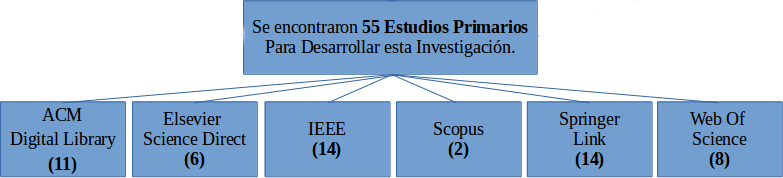
\includegraphics[scale=0.45]{images/1document/seleccionParte2.png}
        			\caption{Estudios Primarios por Biblioteca Digital}
		        	\label{primariosBiblioteca}
           		\end{center}
        	\end{figure}
	
    	    \subsubsection{Síntesis de la Información}

            REDACTAR EL DETALLE DE LOS ESTUDIOS PRIMARIOS ENCONTRADOS.
    	    
            \begin{figure}[H]
        		\begin{center}
        			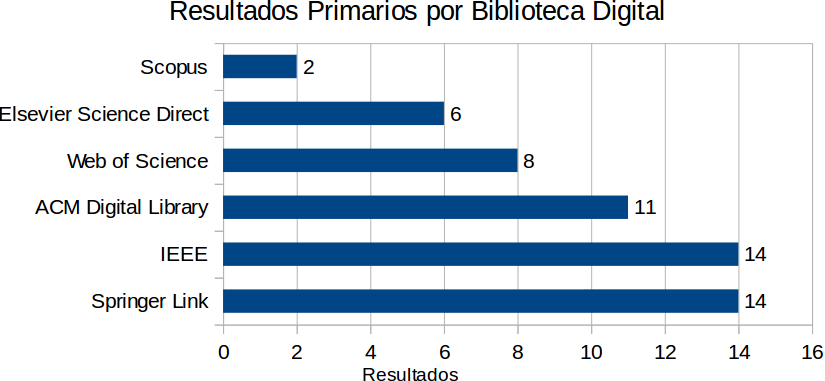
\includegraphics[scale=0.45]{images/1document/PrimariosBD.png}
        			\caption{Estudios Primarios por Biblioteca Digital}
		        	\label{primariosBiblioteca}
           		\end{center}
        	\end{figure}
        	
            \begin{figure}[H]
        		\begin{center}
        			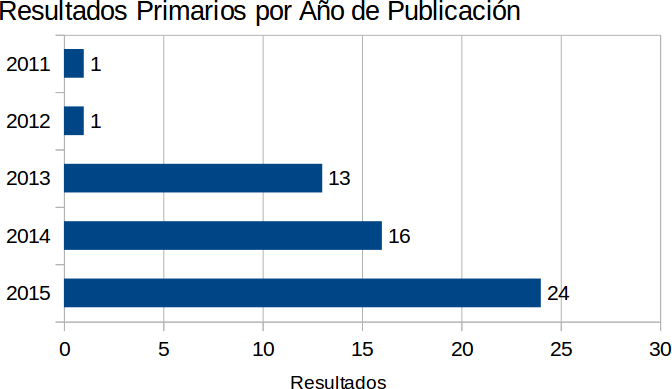
\includegraphics[scale=0.45]{images/1document/PrimariosAnio.png}
        			\caption{Estudios Primarios por Biblioteca Digital}
		        	\label{primariosBiblioteca}
           		\end{center}
        	\end{figure}
        	
            \begin{figure}[H]
        		\begin{center}
        			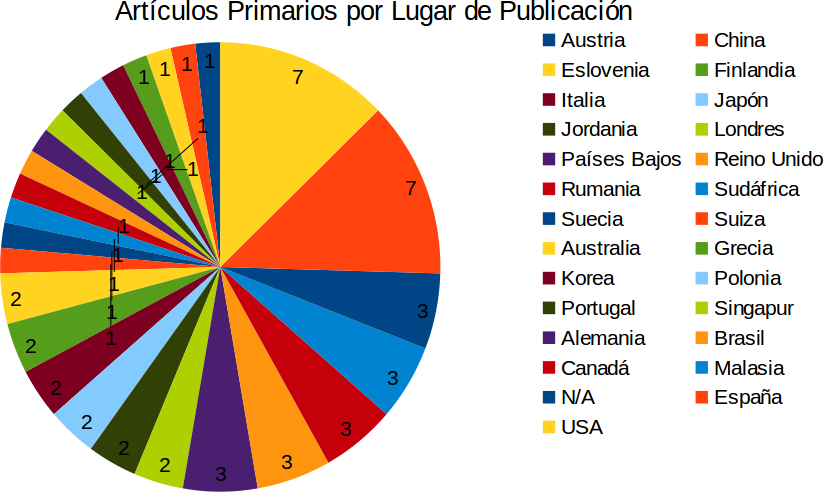
\includegraphics[scale=0.45]{images/1document/PrimariosLugar.png}
        			\caption{Estudios Primarios por Biblioteca Digital}
		        	\label{primariosBiblioteca}
           		\end{center}
        	\end{figure}
    	    
            \begin{figure}[H]
        		\begin{center}
        			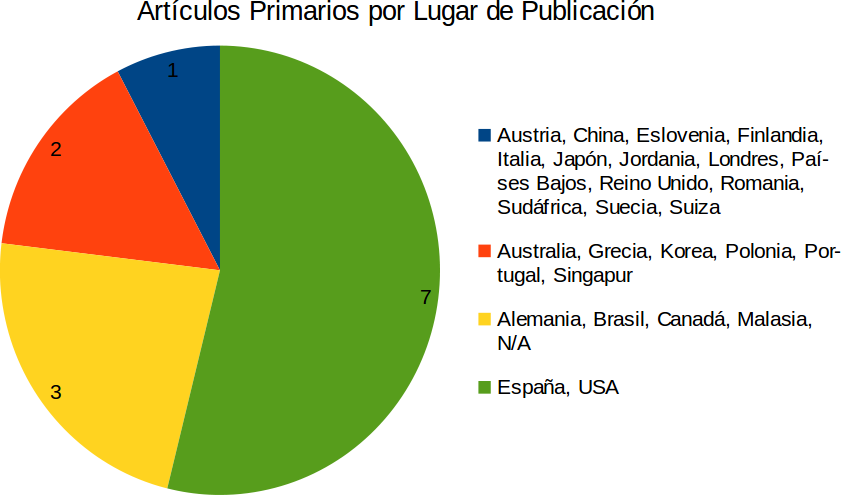
\includegraphics[scale=0.45]{images/1document/PrimariosLugar2.png}
        			\caption{Estudios Primarios por Biblioteca Digital}
		        	\label{primariosBiblioteca}
           		\end{center}
        	\end{figure}
	
	    \subsection{Reporte de Resultados}
	
    	    \subsubsection{Revisiones Literarias}    
    
            \subsubsection{Métodos Existentes}
        
            \subsubsection{Evaluación del Reporte}
        
    \section{Conclusiones}
    
    \newpage
    \bibliographystyle{acm}
    \bibliography{biblist}
    
    
    \section{Anexos}
    AGREGAR LISTA DE REFERENCIAS
    
    
\chapter{Lecciones Aprendidas de una Revisión Sistemática}
    
    \section{Lecciones Aprendidas}
    
    \section{Trabajos Futuros}
    
    \section{conclusiones}

\end{document}
